%!TEX root = ../Electrodynamics.tex
\subsection{Медленные волны, направляемые плоским диэлектрическим слоем. Дифференциальное уравнение для поперечной волновой функции и его решения для областей внутри и вне слоя. Выражения для полей, граничные условия и дисперсионные (характеристические) уравнения для симметричных (чётных) волн типа ТМ}

\begin{figure}[ht]
    \centering
    \incfig{test-fig} 
    \caption{Диэлектрический слой}
    \label{fig:test-fig}
\end{figure}
Рассмотрим задачу о распространении волны вдоль плоского диэлектрического слоя. Так как это бесконечный плоский слой, то $\pdv{y}=0$: $\vec{E},\vec{H} = \vec{E}(t,x,z), \vec{H}(t,x,z)$.
Будем искать решение в виде
\begin{equation}
    \vec{E} = \vec{F}(x) \cdot e^{i(\omega t-hz)} 
\end{equation}
Теперь у нас будут другие граничные условия. Нам придётся решать уравнения Максвелла во всей среде -- в трёх областях: вне слоя сверху, снизу и в слое, а затем сшивать решения.

Введём поперечную волновую функцию $\phi(x)$:
\begin{equation}
    \Delta_\perp \phi  + \kappa^2 \phi = 0, \quad \kappa^2=k_0^2 \varepsilon \mu - h^2
\end{equation}
$h$ должно быть одинаковым в областях 0 (вне слоя) и 1 (в слое), иначе мы заведомо не сможем удовлетворить граничным условиям: количество гребней волн в разных областях не совпадёт. Значит, $h=\const$.

В области 1:
\begin{equation}
    \kappa_1^2 = k_0^2 \varepsilon - h^2, \qquad \dv[2]{\phi}{x}+\kappa_1^2\phi=0
\end{equation}

В области 2:
\begin{equation}
    \kappa_0^2 = k_0^2-h^2, \qquad \dv[2]{\phi}{x}+\kappa_0^2\phi=0
\end{equation}
Отсюда сразу следует, что $\varkappa_1^2 = \varkappa_0^2 + k_0^2(\varepsilon-1)$.

Сначала найдём решение вне слоя. Волна должна быть локализована -- не переносить
энергию в поперечном направлении. Для этого нужно потребовать, чтобы
\begin{equation}
    \kappa_0^2<0 
    \quad\Rightarrow\quad 
    \varkappa_0^2 = -p^2, \quad
    \kappa_0^2 = ip 
    \quad\Rightarrow\quad 
    \phi \sim e^{\pm p x}
\end{equation}
Чтобы удовлетворить локализованности, над слоем должно быть $\phi=c_2 e^{-px}$, а под слоем $\phi=c_2 e^{px}$.

Теперь найдём решение в слое. Пусть $\kappa_1^2>0  \quad\Rightarrow\quad  \varepsilon>1$. Тогда
\begin{equation}
    \phi = A_1 \cos \varkappa_1 x + A_2 \sin \varkappa_1 x
\end{equation}

\paragraph{TM волны в плоском слое.} Запишем поля через волновую функцию, как мы это делали в самом начале курса:
\begin{equation}
    E_z = \frac{\kappa^2}{ik_0 \varepsilon}\phi, \qquad
    E_x = -\frac{h}{k_0 \varepsilon} \dv{\phi}{x}, \qquad
    H_y = -dv{\phi}{x}
\end{equation}
$E_y, H_x$ нет, так как они пропорциональны $\pdv{\phi}{y}=0$.
На границе диэлектрика у нас должны быть непрерывны тангенциальные компоненты полей $E,H$ в точках $x=\pm l$.

Граничное условия для $E_z$ (первая формула) и для $H_y$ (вторая):
\begin{equation}
    \frac{\kappa_1^2 \phi(l-0)}{\varepsilon}, \qquad
    \dv{\phi(l-0)}{x} = \dv{\phi(l+0)}{x}
\end{equation}
\paragraph{Чётные и нечётные волны. } Целесообразно для упрощения расчётов разделять четные волны ($f(x)=f(-x) \Rightarrow \phi = A\sin \kappa_1 x$), и нечётные ($f(x)=-f(x) \Rightarrow \phi=A\cos\kappa_1 x$). Тогда для чётных волн граничные условия примут вид
\begin{equation}
    %x>L: \quad
    \left\{\begin{aligned}
            \frac{1}{\varepsilon}\kappa_1^2 A\sin\kappa_1 l = -p^2 C e^{-pl}\\
            \kappa_1^2 A \cos \kappa_1 l = -p C e^{-pl} 
    \end{aligned}\right.
\end{equation}
Условие разрешимости этой системы -- определитель её равен нулю:
\begin{equation}
    \left\{\begin{aligned}
            &\frac{\varkappa_1 l}{\varepsilon} \tg \kappa_1 l = pl\\
            &(\kappa_1 l)^2 +  (pl)^2 = (k_0 l)^2 (\varepsilon-1)
    \end{aligned}\right.
\end{equation}
Без вывода приведём такие же выражения для нечётных волн:
\begin{equation}
    \left\{\begin{aligned}
        &-\frac{\kappa_1 l}{\varepsilon} \ctg \kappa_1 l = pl\\
        &(\kappa_1 l)^2 +  (pl)^2 = (k_0 l)^2 (\varepsilon-1)
    \end{aligned}\right.
\end{equation}
Это трансцендентные уравнения, и просто так их решить нельзя. Но в этом случае оказывается целесообразным применить графический метод решения, который даст нам ключевую информацию о появлении мод. Построим оба уравнения в координатах $(pl, \varkappa_1 l)$:
\begin{figure}[H]
    \centering
    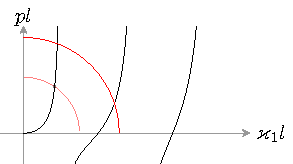
\includegraphics[scale=1.5]{img3/1}
    \caption{Появление мод}
    \label{fig:}
\end{figure}
Здесь радиус окружности $E=k_0 l \sqrt{\varepsilon-1}$. Если $R<\pi$, то есть только один корень: мода ТМ${}_{00}$. Когда окружность пересекает функцию в $pl=0$, это критическая частота данной моды: так как $p=0$ отвечает нелокализованной моде. Первый индекс моды связан с количеством корней уравнения, а второй у нас будет всегда 0 -- мы не рассматривали зависимость от $y$.
\paragraph{Низшая мода TM${}_{00}$.} Построим графики поперечного распределения поля:
\begin{figure}[H]
    \centering
    \incfigg{00}{1}
    \caption{Поле $H_y$ непрерывно, а $E_z$ терпит скачок, так как непрерывна $D_n$}
    \label{fig:hytm00}
\end{figure}

\paragraph{ТЕ-волны.} Для них
\begin{equation}
    \qq{чет:} \varkappa_1 l \tg \varkappa_1 l = pl, \quad
    \qq{нечет:} -\varkappa_1 l \ctg \varkappa_1 l = pl
\end{equation}
ТЕ волны возможны, только если $R>\frac{m\pi}{2}$.

\paragraph{Медленные волны. } Почему мы называем эти волны медленными? Посмотрим на дисперсионное уравнение:
\begin{equation}
    k^2 = \frac{\omega^2}{c^2}\varepsilon\mu + p^2 > k^2 
    \quad\Rightarrow\quad 
    v_\text{f}=\frac{\omega}{h} < \frac{\omega}{k}=c.
\end{equation}
Эти волны медленные относительно волн в вакууме: фазовая скорость меньше скорости света.










\newpage
\subsection{Главные (ТЕМ) волны в линиях передач. Условие существования ТЕМ волны. ТЕМ волна в коаксиальной линии (Картинка силовых линий, зависимость полей от координат).}

%Главные (TEM) волны в линиях передачи с идеальными границами

У TEM-волн поперечное волновое число $\varkappa=0$:
\begin{equation*}
\varkappa=0 \Rightarrow h=k= \frac{\omega}{c}\sqrt{\varepsilon \mu}
\end{equation*}
Поля таких волн выражаются следующим образом через функцию $\varphi$:
\begin{gather*}
\label{eperp}
\vec{E}_\perp=-\frac{1}{\sqrt{\varepsilon \mu}}\nabla_\perp \varphi\\
\vec{H}_\perp=-\frac{1}{\mu}\qty[\nabla_\perp \varphi,\vec{z}_0]
\end{gather*}

При этом выполняются \textbf{граничные условия}: на каждом из проводников (допустим, есть набор проводников, вдоль которых распространяется волна)
\begin{equation*}
\varphi|_{l_i}=C_i,
\end{equation*}
причем константа не обязана быть одна для всех проводников.

\begin{figure}[H]
	\centering
	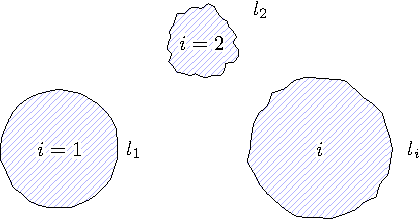
\includegraphics[scale=1]{img/lect4_ris1}
	\caption{Набор проводников в задаче}
	\label{fig:lect4:1}
\end{figure}

\paragraph{Внутренняя задача.} Пусть у нас есть только один проводник, в котором есть цилиндрическая полость (рис. \ref{fig:lect4:2}). Рассмотрим внутреннюю задачу, т.е. распространение волны внутри цилиндрической полости.  
\begin{figure}[H]
	\centering
	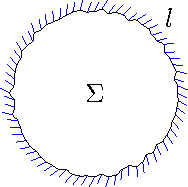
\includegraphics[scale=1]{img/lect4_ris2}
	\caption{Случай одного проводника}
	\label{fig:lect4:2}
\end{figure}
Оказывается, для граничного условия $\varphi_\perp|_l=C_1$ существует только тривиальное решение $\varphi_\perp=C_1$. Для доказательства необходимо воспользоваться теоремой и минимуме и максимуме для гармонической функции.
%\begin{equation*}
%\Delta \varphi=\Div\qty(\varphi\nabla \varphi)=0 \quad \bigg| \iint\limits_\Sigma
%\end{equation*}
%Это такая задача, которую проще доказать самому. Попробуйте это сделать сами.

\paragraph{Внешняя задача. } Зададимся вопросом о решении той же задачи:
\begin{equation*}
\Delta_\perp \varphi=0, \quad \varphi|_l=\mathrm{const}
\end{equation*}
Только теперь будем рассматривать её в области вне проводника

Для начала рассмотрим задачу попроще, поле нити (рис. \ref{fig:lect4:3}). Её решение известно:
\begin{equation*}
\Delta_\perp \varphi=0 
\quad \Rightarrow \quad
\varphi \sim \ln r
\end{equation*} 

Характер убывания полей здесь $\displaystyle E_r\sim \frac{1}{r}$, а для магнитного поля в силу импедансного соотношения
$\displaystyle\frac{E_r}{H_\phi}=\eta_{\perp\text{в}}=1, \quad H_\varphi\sim\frac{1}{r}$:
\begin{equation*} 
E_r=H_\phi\sim\frac{1}{r}
\end{equation*}
\begin{figure}[H]
	\centering
	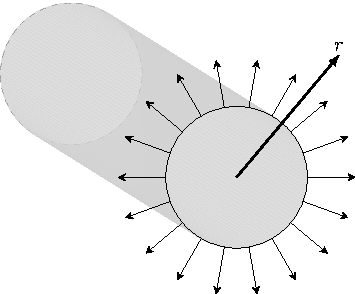
\includegraphics[width =0.4\linewidth]{img/lect4_ris3}
	\caption{Поле бесконечной проводящей нити}
	\label{fig:lect4:3}
\end{figure}

Посмотрим на поведение полей при $r\to\infty$. Говорят, нужно поставить граничные условия (или закон убывания) на
бесконечности. Чем плох закон $\frac{1}{r}$?

Посчитаем средний по времени поток энергии через поперечное сечение, в котором распространяется волна. Сечение
бесконечно, за исключением конечной площади проводника.

Сначала вычислим вектор Пойнтинга (средний по времени и в проекции на $z$):
\begin{equation*}
\overline{S}_z=\frac{c}{8 \pi}\mathrm{Re}\qty(E_r\cdot H_\phi^*)\sim\frac{1}{r^2}
\end{equation*}
\begin{equation*}
\Pi=\iint\limits_\Sigma \overline{S}_z ds \sim
\iint\limits_\Sigma \frac{1}{r^2} (2\pi r \dd{r})
\sim \int\limits_a^\infty = \ln\frac{\infty}{a}=\infty
\end{equation*}
Интеграл расходится на бесконечности. Говорят, что расходимость носит логарифмический характер. Получили бесконечную мощность волны: такую волну невозможно создать реальным источником --- волна не удовлетворяет критерию энергетической реализуемости.

Можно сделать важный вывод: \textbf{вдоль одиночного проводника TEM-волна с конечной энергией распространятся не может}. Распространение возможно, если количество проводников будет больше одного. Например, в линии из двух проводников (рис. \ref{fig:lect4:4}) TEM-волна уже возможна.

\begin{figure}[h!]
	\centering
	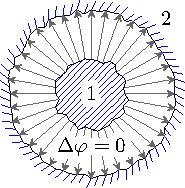
\includegraphics[scale=1.5]{img/lect4_ris4}
	\caption{Закрытая линия из двух проводников}
	\label{fig:lect4:4}
\end{figure}

Можно модифицировать задачу с нитью (рис. \ref{fig:lect4:5}):

\begin{figure}[h!]
	\centering
	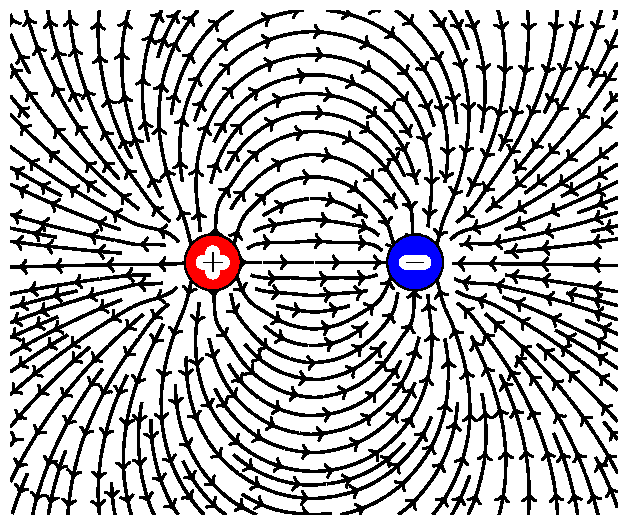
\includegraphics[scale=0.7]{img/lect4_ris5}
	\caption{Поле двухпроводной линии}
	\label{fig:lect4:5}
\end{figure}

В поперечном разрезе это поле диполя, а оно спадает быстрее, $\sim \frac{1}{r^2}$. Тогда
\begin{equation*}
E_\perp\sim H_\perp \sim \frac{1}{r^2}
\quad \Rightarrow \quad
\overline{S}_z \sim \frac{1}{r^4}, \quad
\Pi \sim \int\limits_{L_\text{характ}}^\infty \frac{1}{r^3} \dd{r}
\end{equation*}

Мощность волны конечна, значит, в модифицированной задаче TEM-волна энергетически реализуема.

\textbf{Конечный вывод:} TEM-волна в идеальной линии передачи возможна, если число проводников $\geq 2$.

Например, в коаксиальной линии (рис. \ref{fig:lect4:6}) TEM-волна возможна.

\begin{figure}[h!]
	\centering
	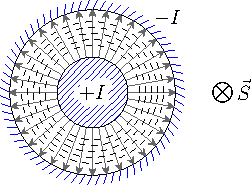
\includegraphics[scale=1.5]{img/lect4_ris6}
	\caption{Поле в коаксиальном кабеле}
	\label{fig:lect4:6}
\end{figure}

Зададимся вопросом: возможны ли в такой линии TE и TM волны? Сформулируем утверждение, пока без доказательства:
\textbf{в открытых линиях передачи TE и TM волны не существуют}.
